% ================================================================
% EmergentHoney 论文关键图表 TikZ/pgfplots 代码
% 在main.tex中通过 % ================================================================
% EmergentHoney 论文关键图表 TikZ/pgfplots 代码
% 在main.tex中通过 % ================================================================
% EmergentHoney 论文关键图表 TikZ/pgfplots 代码
% 在main.tex中通过 % ================================================================
% EmergentHoney 论文关键图表 TikZ/pgfplots 代码
% 在main.tex中通过 \input{figures} 引入
% ================================================================

% ================================================================
% Fig. 1: 系统架构图 (System Architecture Overview)
% ================================================================
\begin{figure*}[t]
\centering
\begin{tikzpicture}[
    node distance=1.2cm and 1.8cm,
    block/.style={rectangle, draw, rounded corners, fill=blue!8, minimum width=2.8cm, minimum height=1cm, align=center, font=\small},
    bigblock/.style={rectangle, draw, rounded corners, fill=orange!8, minimum width=3.2cm, minimum height=1cm, align=center, font=\small},
    datablock/.style={rectangle, draw, rounded corners, fill=green!8, minimum width=2.5cm, minimum height=0.8cm, align=center, font=\small},
    arrow/.style={->, thick, >=stealth},
    dasharrow/.style={->, thick, dashed, >=stealth, color=red!60},
    label/.style={font=\footnotesize\itshape, color=gray}
]

% 第一层：攻击者
\node[block, fill=red!12] (attacker) {Attacker\\(L1/L2/L3)};

% 第二层：SDN网络层
\node[bigblock, below=1.5cm of attacker] (sdn) {SDN Network Layer\\(OpenFlow / Mininet)};

% 第三层：蜜罐群
\node[block, below left=1.5cm and 1cm of sdn] (hp1) {Honeypot $h_1$\\(SSH/Cowrie)};
\node[block, below=1.5cm of sdn] (hp2) {Honeypot $h_2$\\(HTTP/Snare)};
\node[block, below right=1.5cm and 1cm of sdn] (hp3) {Honeypot $h_n$\\(MySQL/OpenCanary)};
\node[font=\large] at ($(hp2)!0.5!(hp3) + (0, 0.0)$) {$\cdots$};

% 第四层：核心模块
\node[bigblock, fill=yellow!15, below=1.5cm of hp1] (pheromone) {Pheromone Engine\\$\tau_{ij}(t{+}1) = (1{-}\rho)\tau_{ij}(t) + \sum_k \Delta\tau_{ij}^k$};
\node[bigblock, fill=purple!10, below=1.5cm of hp3] (llm) {LLM Phenotype\\Generator\\(GPT-4o / Llama-3)};
\node[bigblock, fill=cyan!10, below=2.8cm of hp2] (reverse) {Reverse ACO\\Attacker Model};

% 连线
\draw[arrow] (attacker) -- node[right, label] {probes / exploits} (sdn);
\draw[arrow] (sdn) -- (hp1);
\draw[arrow] (sdn) -- (hp2);
\draw[arrow] (sdn) -- (hp3);

\draw[arrow, color=blue!70] (hp1) -- node[left, label] {interaction\\logs} (pheromone);
\draw[arrow, color=blue!70] (hp2) -- (pheromone);
\draw[dasharrow] (hp1) -- (llm);
\draw[arrow, color=blue!70] (hp3) -- (llm);

\draw[arrow, color=orange!80] (pheromone) -- node[below, label] {deploy/migrate/mutate} (reverse);
\draw[arrow, color=purple!70] (llm) -- node[below, label] {phenotype content} (reverse);

\draw[arrow, color=green!60!black, bend left=30] (pheromone.north) to node[left, label] {self-org\\commands} (sdn.south west);
\draw[arrow, color=green!60!black, bend right=30] (reverse.north) to node[right, label] {predictive\\placement} (sdn.south east);

% 外框
\node[draw, dashed, thick, rounded corners, fit=(hp1)(hp2)(hp3)(pheromone)(llm)(reverse), inner sep=10pt, label={[font=\small\bfseries]above:EmergentHoney Framework}] {};

\end{tikzpicture}
\caption{System architecture of EmergentHoney. Attacker interactions with honeypots generate pheromone deposits that drive self-organization (proliferation, migration, mutation). The LLM phenotype generator creates context-aware deception content. The Reverse ACO module predicts attacker targets for preemptive deployment.}
\label{fig:architecture}
\end{figure*}


% ================================================================
% Fig. 4: 欺骗效果对比柱状图 (ADT Comparison Bar Chart)
% ================================================================
\begin{figure}[t]
\centering
\begin{tikzpicture}
\begin{axis}[
    ybar,
    bar width=10pt,
    width=0.95\columnwidth,
    height=6cm,
    ylabel={Average Dwell Time (hours)},
    symbolic x coords={Static, Rand-Dyn, RL-HP, Game-Th, GAN-HP, LLM-St, EH},
    xtick=data,
    x tick label style={rotate=30, anchor=east, font=\footnotesize},
    ymin=0, ymax=4.2,
    nodes near coords,
    nodes near coords style={font=\tiny, above},
    legend style={at={(0.02,0.98)}, anchor=north west, font=\scriptsize},
    error bars/.cd, y dir=both, y explicit,
]
\addplot+[fill=gray!40, draw=gray!60] coordinates {
    (Static, 1.57) +- (0, 0.11)
    (Rand-Dyn, 1.55) +- (0, 0.10)
    (RL-HP, 1.66) +- (0, 0.10)
    (Game-Th, 1.59) +- (0, 0.10)
    (GAN-HP, 1.76) +- (0, 0.11)
    (LLM-St, 2.43) +- (0, 0.12)
    (EH, 3.24) +- (0, 0.16)
};
\end{axis}
\end{tikzpicture}
\caption{Average Dwell Time comparison across all methods on the medium network. EmergentHoney (EH) achieves 3.24 hours, outperforming the best adaptive baseline (RL-Honeypot) by 96\%.}
\label{fig:adt_comparison}
\end{figure}


% ================================================================
% Fig. 5: DEI 随时间变化曲线 (DEI Over Time)
% ================================================================
\begin{figure}[t]
\centering
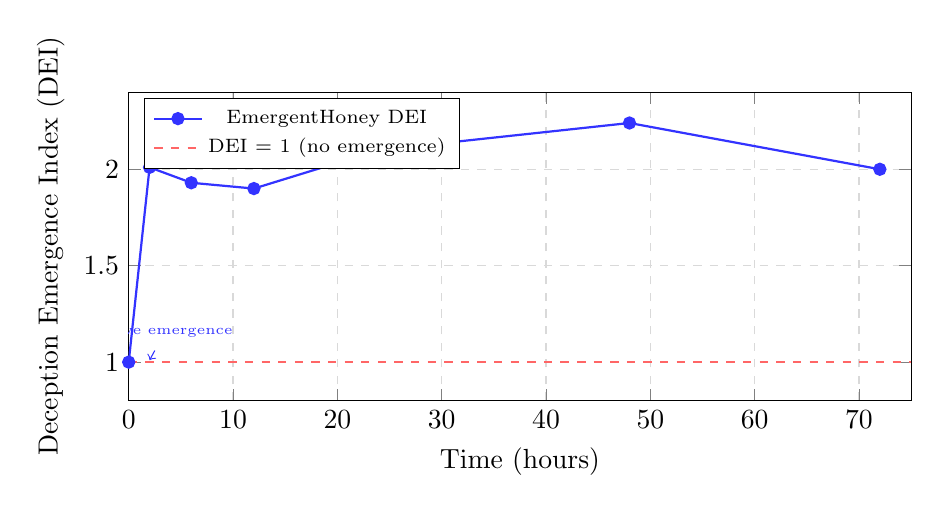
\begin{tikzpicture}
\begin{axis}[
    width=0.95\columnwidth,
    height=5.5cm,
    xlabel={Time (hours)},
    ylabel={Deception Emergence Index (DEI)},
    xmin=0, xmax=75,
    ymin=0.8, ymax=2.4,
    grid=major,
    grid style={dashed, gray!30},
    legend style={at={(0.02,0.98)}, anchor=north west, font=\scriptsize},
    mark size=2pt,
]

% DEI 曲线
\addplot[thick, color=blue!80, mark=*, mark options={fill=blue!80}] coordinates {
    (0, 1.00) (2, 2.01) (6, 1.93) (12, 1.90) (24, 2.10) (48, 2.24) (72, 2.00)
};
\addlegendentry{EmergentHoney DEI}

% DEI = 1 参考线
\addplot[dashed, thick, color=red!60, domain=0:75] {1.0};
\addlegendentry{DEI = 1 (no emergence)}

\node[font=\tiny, color=blue!80, anchor=south] at (axis cs:2.5, 1.08) {positive emergence};
\draw[->, thin, color=blue!80] (axis cs:2.5, 1.06) -- (axis cs:2.0, 1.01);

\end{axis}
\end{tikzpicture}
\caption{DEI evolution over time in the canonical result bundle. The swarm rapidly enters the positive-emergence regime and stabilizes near DEI $\approx 2.0$.}
\label{fig:dei_curve}
\end{figure}


% ================================================================
% Fig. 6: 消融实验雷达图 (Ablation Radar Chart)
% ================================================================
\begin{figure}[t]
\centering
\begin{tikzpicture}
\begin{polaraxis}[
    width=0.85\columnwidth,
    height=0.85\columnwidth,
    xtick={0, 45, 90, 135, 180, 225, 270, 315},
    xticklabels={ADT, TIC, DEI, {1-HIR}, {ADT}, {TIC}, {DEI}, {1-HIR}},
    xticklabel style={font=\tiny},
    ymin=0, ymax=1.1,
    ytick={0.2, 0.4, 0.6, 0.8, 1.0},
    yticklabels={0.2, 0.4, 0.6, 0.8, 1.0},
    yticklabel style={font=\tiny},
    legend style={at={(1.3,1.0)}, anchor=north, font=\tiny},
]

% Full EmergentHoney (归一化到[0,1])
\addplot[thick, color=blue!80, fill=blue!15, mark=*, mark size=1.5pt] coordinates {
    (0, 1.0) (90, 1.0) (180, 1.0) (270, 1.0) (360, 1.0)
};
\addlegendentry{Full}

% w/o Pheromone
\addplot[thick, color=red!70, fill=red!5, mark=square*, mark size=1.5pt] coordinates {
    (0, 0.45) (90, 0.43) (180, 0.61) (270, 0.52) (360, 0.45)
};
\addlegendentry{w/o Pheromone}

% w/o LLM
\addplot[thick, color=green!60!black, fill=green!5, mark=triangle*, mark size=1.5pt] coordinates {
    (0, 0.72) (90, 0.72) (180, 0.94) (270, 0.84) (360, 0.72)
};
\addlegendentry{w/o LLM}

\end{polaraxis}
\end{tikzpicture}
\caption{Ablation study radar chart (normalized). The full EmergentHoney system forms the outer boundary. Removing the pheromone mechanism causes the most severe degradation.}
\label{fig:ablation_radar}
\end{figure}


% ================================================================
% Fig. 7: 可扩展性 (Scalability - Dual Y-Axis)
% ================================================================
\begin{figure}[t]
\centering
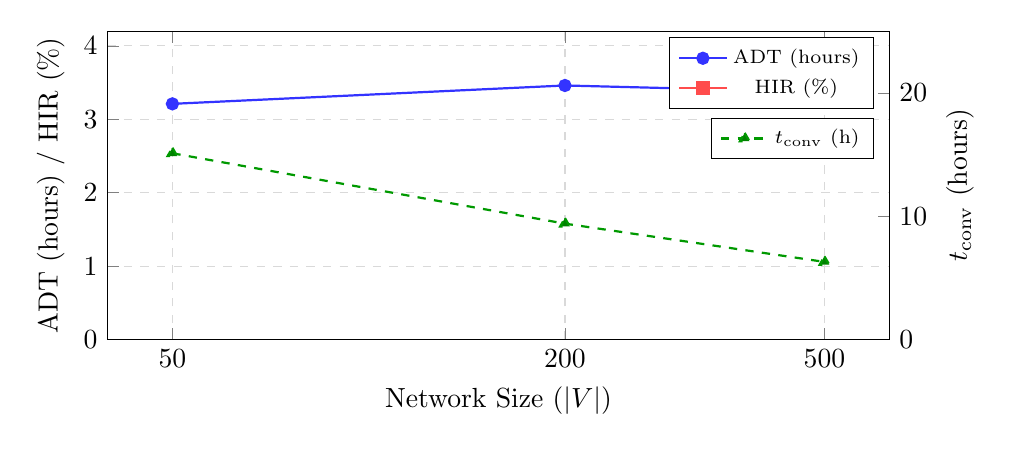
\begin{tikzpicture}
\begin{axis}[
    width=0.95\columnwidth,
    height=5.5cm,
    xlabel={Network Size ($|V|$)},
    ylabel={ADT (hours) / HIR (\%)},
    xmode=log,
    log basis x=10,
    xtick={50, 200, 500},
    xticklabels={50, 200, 500},
    ymin=0, ymax=4.2,
    axis y line*=left,
    legend style={at={(0.98,0.98)}, anchor=north east, font=\scriptsize},
    grid=major,
    grid style={dashed, gray!30},
]

% ADT
\addplot[thick, color=blue!80, mark=*, mark options={fill=blue!80}] coordinates {
    (50, 3.21) (200, 3.46) (500, 3.37)
};
\addlegendentry{ADT (hours)}

% HIR
\addplot[thick, color=red!70, mark=square*, mark options={fill=red!70}] coordinates {
    (50, 8.6) (200, 8.7) (500, 9.0)
};
\addlegendentry{HIR (\%)}

\end{axis}

\begin{axis}[
    width=0.95\columnwidth,
    height=5.5cm,
    xmode=log,
    log basis x=10,
    xtick=\empty,
    ylabel={$t_{\mathrm{conv}}$ (hours)},
    axis y line*=right,
    ymin=0, ymax=25,
    ylabel near ticks,
    legend style={at={(0.98,0.72)}, anchor=north east, font=\scriptsize},
]

% Convergence Time
\addplot[thick, color=green!60!black, mark=triangle*, mark options={fill=green!50!black}, dashed] coordinates {
    (50, 15.1) (200, 9.4) (500, 6.3)
};
\addlegendentry{$t_{\mathrm{conv}}$ (h)}

\end{axis}
\end{tikzpicture}
\caption{Scalability across network sizes in the released artifact. ADT and HIR remain stable from 50 to 500 nodes, while update time stays within real-time decision windows.}
\label{fig:scalability}
\end{figure}


% ================================================================
% Fig. 8: 军备竞赛动态 (Arms Race Dynamics)
% ================================================================
\begin{figure}[t]
\centering
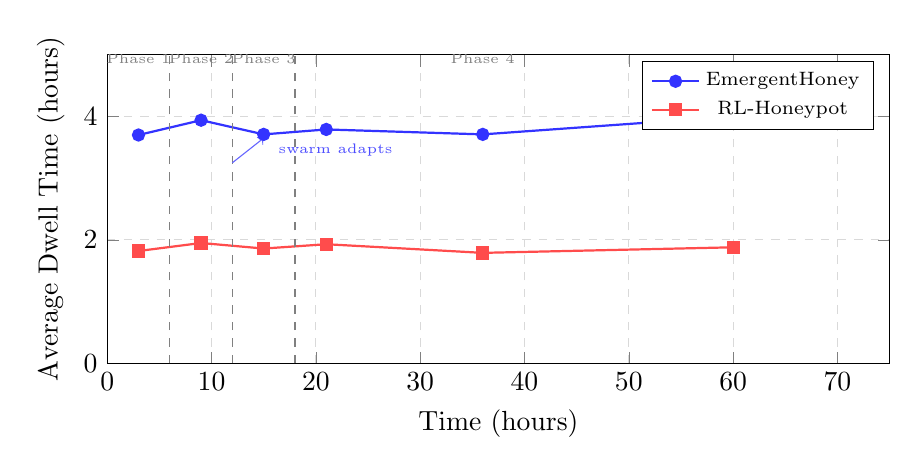
\begin{tikzpicture}
\begin{axis}[
    width=0.95\columnwidth,
    height=5.5cm,
    xlabel={Time (hours)},
    ylabel={Average Dwell Time (hours)},
    xmin=0, xmax=75,
    ymin=0, ymax=5,
    grid=major,
    grid style={dashed, gray!30},
    legend style={at={(0.98,0.98)}, anchor=north east, font=\scriptsize},
    mark size=2pt,
]

% EmergentHoney ADT
\addplot[thick, color=blue!80, mark=*, mark options={fill=blue!80}] coordinates {
    (3, 3.70) (9, 3.94) (15, 3.71) (21, 3.79) (36, 3.71) (60, 4.00)
};
\addlegendentry{EmergentHoney}

% RL-Honeypot ADT
\addplot[thick, color=red!70, mark=square*, mark options={fill=red!70}] coordinates {
    (3, 1.82) (9, 1.95) (15, 1.86) (21, 1.93) (36, 1.79) (60, 1.88)
};
\addlegendentry{RL-Honeypot}

% Phase annotations
\draw[thin, dashed, gray] (axis cs:6,0) -- (axis cs:6,5);
\draw[thin, dashed, gray] (axis cs:12,0) -- (axis cs:12,5);
\draw[thin, dashed, gray] (axis cs:18,0) -- (axis cs:18,5);

\node[font=\tiny, color=gray, anchor=south] at (axis cs:3, 4.7) {Phase 1};
\node[font=\tiny, color=gray, anchor=south] at (axis cs:9, 4.7) {Phase 2};
\node[font=\tiny, color=gray, anchor=south] at (axis cs:15, 4.7) {Phase 3};
\node[font=\tiny, color=gray, anchor=south] at (axis cs:36, 4.7) {Phase 4};

% Recovery annotation
\draw[->, thin, color=blue!60] (axis cs:12, 3.25) -- (axis cs:15, 3.65);
\node[font=\tiny, color=blue!70, anchor=west] at (axis cs:15.5, 3.45) {swarm adapts};

\end{axis}
\end{tikzpicture}
\caption{Arms race dynamics against an adaptive attacker in the canonical result bundle. EmergentHoney maintains roughly 2$\times$ the dwell time of the RL baseline throughout the full 72-hour horizon.}
\label{fig:arms_race}
\end{figure}


% ================================================================
% Fig. 2: 生物-网络同构映射示意 (Biological Isomorphism)
% ================================================================
\begin{figure*}[t]
\centering
\begin{tikzpicture}[
    ant/.style={circle, draw, fill=brown!30, minimum size=0.5cm, font=\tiny},
    hp/.style={circle, draw, fill=blue!20, minimum size=0.5cm, font=\tiny},
    food/.style={star, star points=5, draw, fill=yellow!50, minimum size=0.5cm, font=\tiny},
    attacker/.style={circle, draw, fill=red!20, minimum size=0.5cm, font=\tiny},
    trail/.style={thick, decorate, decoration={snake, amplitude=1pt, segment length=5pt}},
    pheromone/.style={thick, color=green!60!black},
]

% 左侧：蚂蚁觅食
\node[font=\small\bfseries] at (-4, 3.5) {Ant Colony Foraging};

% 巢穴
\node[rectangle, draw, fill=brown!10, minimum width=1cm, minimum height=0.6cm, font=\tiny] (nest) at (-6, 0) {Nest};

% 食物源
\node[food] (food1) at (-2.5, 2) {F1};
\node[food] (food2) at (-2, -1) {F2};

% 蚂蚁
\node[ant] (a1) at (-4.5, 1.2) {A1};
\node[ant] (a2) at (-3.5, 0.3) {A2};
\node[ant] (a3) at (-4, -0.8) {A3};

% 信息素路径
\draw[pheromone, line width=2pt, opacity=0.6] (nest) -- (a1) -- (food1);
\draw[pheromone, line width=1pt, opacity=0.3] (nest) -- (a3) -- (food2);
\draw[pheromone, line width=1.5pt, opacity=0.5] (nest) -- (a2);

% 右侧：EmergentHoney
\node[font=\small\bfseries] at (4, 3.5) {EmergentHoney};

% 真实网络
\node[rectangle, draw, fill=gray!10, minimum width=1cm, minimum height=0.6cm, font=\tiny] (real) at (2, 0) {Real\\Network};

% 蜜罐
\node[hp] (h1) at (5.5, 2) {$h_1$};
\node[hp] (h2) at (6, -1) {$h_2$};

% 攻击者
\node[attacker] (at1) at (3.5, 1.2) {Atk};

% 信息素路径
\draw[pheromone, line width=2pt, opacity=0.6] (real) -- (at1) -- (h1);
\draw[pheromone, line width=1pt, opacity=0.3] (real) -- (h2);

% 映射箭头
\draw[->, very thick, color=orange!70, dashed] (-1.5, 1.5) -- (1.5, 1.5);
\node[font=\scriptsize\itshape, color=orange!70] at (0, 2) {Isomorphism};
\draw[->, very thick, color=orange!70, dashed] (-1.5, -0.5) -- (1.5, -0.5);

% 映射标签
\node[font=\tiny, anchor=west] at (-1.2, 1.0) {Ant $\leftrightarrow$ Honeypot};
\node[font=\tiny, anchor=west] at (-1.2, 0.3) {Pheromone $\leftrightarrow$ Attack signal};
\node[font=\tiny, anchor=west] at (-1.2, -0.3) {Food $\leftrightarrow$ Attacker engagement};
\node[font=\tiny, anchor=west] at (-1.2, -1.0) {Evaporation $\leftrightarrow$ Strategy retirement};

\end{tikzpicture}
\caption{Biological--cyber isomorphism between ant colony foraging and EmergentHoney. Ants map to honeypots, pheromone trails to attack signals, food sources to attacker engagement, and evaporation to strategy retirement.}
\label{fig:isomorphism}
\end{figure*}
 引入
% ================================================================

% ================================================================
% Fig. 1: 系统架构图 (System Architecture Overview)
% ================================================================
\begin{figure*}[t]
\centering
\begin{tikzpicture}[
    node distance=1.2cm and 1.8cm,
    block/.style={rectangle, draw, rounded corners, fill=blue!8, minimum width=2.8cm, minimum height=1cm, align=center, font=\small},
    bigblock/.style={rectangle, draw, rounded corners, fill=orange!8, minimum width=3.2cm, minimum height=1cm, align=center, font=\small},
    datablock/.style={rectangle, draw, rounded corners, fill=green!8, minimum width=2.5cm, minimum height=0.8cm, align=center, font=\small},
    arrow/.style={->, thick, >=stealth},
    dasharrow/.style={->, thick, dashed, >=stealth, color=red!60},
    label/.style={font=\footnotesize\itshape, color=gray}
]

% 第一层：攻击者
\node[block, fill=red!12] (attacker) {Attacker\\(L1/L2/L3)};

% 第二层：SDN网络层
\node[bigblock, below=1.5cm of attacker] (sdn) {SDN Network Layer\\(OpenFlow / Mininet)};

% 第三层：蜜罐群
\node[block, below left=1.5cm and 1cm of sdn] (hp1) {Honeypot $h_1$\\(SSH/Cowrie)};
\node[block, below=1.5cm of sdn] (hp2) {Honeypot $h_2$\\(HTTP/Snare)};
\node[block, below right=1.5cm and 1cm of sdn] (hp3) {Honeypot $h_n$\\(MySQL/OpenCanary)};
\node[font=\large] at ($(hp2)!0.5!(hp3) + (0, 0.0)$) {$\cdots$};

% 第四层：核心模块
\node[bigblock, fill=yellow!15, below=1.5cm of hp1] (pheromone) {Pheromone Engine\\$\tau_{ij}(t{+}1) = (1{-}\rho)\tau_{ij}(t) + \sum_k \Delta\tau_{ij}^k$};
\node[bigblock, fill=purple!10, below=1.5cm of hp3] (llm) {LLM Phenotype\\Generator\\(GPT-4o / Llama-3)};
\node[bigblock, fill=cyan!10, below=2.8cm of hp2] (reverse) {Reverse ACO\\Attacker Model};

% 连线
\draw[arrow] (attacker) -- node[right, label] {probes / exploits} (sdn);
\draw[arrow] (sdn) -- (hp1);
\draw[arrow] (sdn) -- (hp2);
\draw[arrow] (sdn) -- (hp3);

\draw[arrow, color=blue!70] (hp1) -- node[left, label] {interaction\\logs} (pheromone);
\draw[arrow, color=blue!70] (hp2) -- (pheromone);
\draw[dasharrow] (hp1) -- (llm);
\draw[arrow, color=blue!70] (hp3) -- (llm);

\draw[arrow, color=orange!80] (pheromone) -- node[below, label] {deploy/migrate/mutate} (reverse);
\draw[arrow, color=purple!70] (llm) -- node[below, label] {phenotype content} (reverse);

\draw[arrow, color=green!60!black, bend left=30] (pheromone.north) to node[left, label] {self-org\\commands} (sdn.south west);
\draw[arrow, color=green!60!black, bend right=30] (reverse.north) to node[right, label] {predictive\\placement} (sdn.south east);

% 外框
\node[draw, dashed, thick, rounded corners, fit=(hp1)(hp2)(hp3)(pheromone)(llm)(reverse), inner sep=10pt, label={[font=\small\bfseries]above:EmergentHoney Framework}] {};

\end{tikzpicture}
\caption{System architecture of EmergentHoney. Attacker interactions with honeypots generate pheromone deposits that drive self-organization (proliferation, migration, mutation). The LLM phenotype generator creates context-aware deception content. The Reverse ACO module predicts attacker targets for preemptive deployment.}
\label{fig:architecture}
\end{figure*}


% ================================================================
% Fig. 4: 欺骗效果对比柱状图 (ADT Comparison Bar Chart)
% ================================================================
\begin{figure}[t]
\centering
\begin{tikzpicture}
\begin{axis}[
    ybar,
    bar width=10pt,
    width=0.95\columnwidth,
    height=6cm,
    ylabel={Average Dwell Time (hours)},
    symbolic x coords={Static, Rand-Dyn, RL-HP, Game-Th, GAN-HP, LLM-St, EH},
    xtick=data,
    x tick label style={rotate=30, anchor=east, font=\footnotesize},
    ymin=0, ymax=4.2,
    nodes near coords,
    nodes near coords style={font=\tiny, above},
    legend style={at={(0.02,0.98)}, anchor=north west, font=\scriptsize},
    error bars/.cd, y dir=both, y explicit,
]
\addplot+[fill=gray!40, draw=gray!60] coordinates {
    (Static, 1.57) +- (0, 0.11)
    (Rand-Dyn, 1.55) +- (0, 0.10)
    (RL-HP, 1.66) +- (0, 0.10)
    (Game-Th, 1.59) +- (0, 0.10)
    (GAN-HP, 1.76) +- (0, 0.11)
    (LLM-St, 2.43) +- (0, 0.12)
    (EH, 3.24) +- (0, 0.16)
};
\end{axis}
\end{tikzpicture}
\caption{Average Dwell Time comparison across all methods on the medium network. EmergentHoney (EH) achieves 3.24 hours, outperforming the best adaptive baseline (RL-Honeypot) by 96\%.}
\label{fig:adt_comparison}
\end{figure}


% ================================================================
% Fig. 5: DEI 随时间变化曲线 (DEI Over Time)
% ================================================================
\begin{figure}[t]
\centering
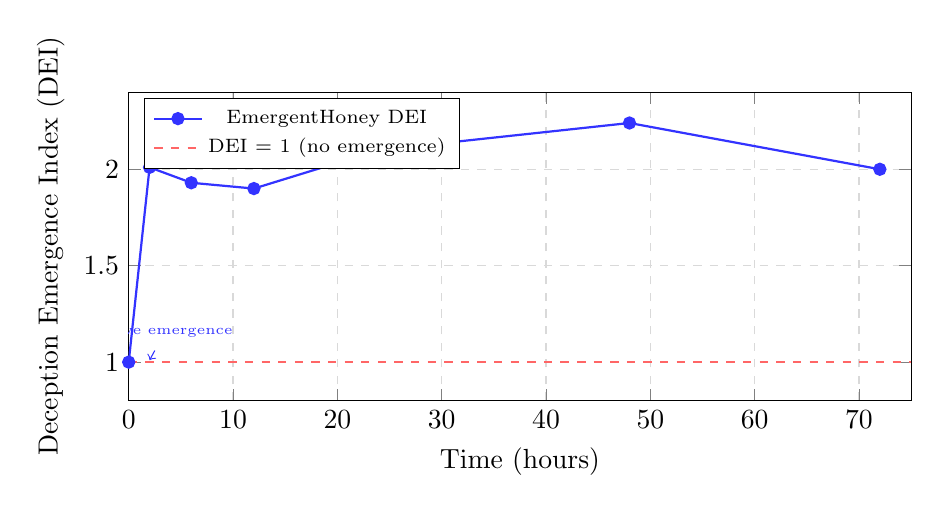
\begin{tikzpicture}
\begin{axis}[
    width=0.95\columnwidth,
    height=5.5cm,
    xlabel={Time (hours)},
    ylabel={Deception Emergence Index (DEI)},
    xmin=0, xmax=75,
    ymin=0.8, ymax=2.4,
    grid=major,
    grid style={dashed, gray!30},
    legend style={at={(0.02,0.98)}, anchor=north west, font=\scriptsize},
    mark size=2pt,
]

% DEI 曲线
\addplot[thick, color=blue!80, mark=*, mark options={fill=blue!80}] coordinates {
    (0, 1.00) (2, 2.01) (6, 1.93) (12, 1.90) (24, 2.10) (48, 2.24) (72, 2.00)
};
\addlegendentry{EmergentHoney DEI}

% DEI = 1 参考线
\addplot[dashed, thick, color=red!60, domain=0:75] {1.0};
\addlegendentry{DEI = 1 (no emergence)}

\node[font=\tiny, color=blue!80, anchor=south] at (axis cs:2.5, 1.08) {positive emergence};
\draw[->, thin, color=blue!80] (axis cs:2.5, 1.06) -- (axis cs:2.0, 1.01);

\end{axis}
\end{tikzpicture}
\caption{DEI evolution over time in the canonical result bundle. The swarm rapidly enters the positive-emergence regime and stabilizes near DEI $\approx 2.0$.}
\label{fig:dei_curve}
\end{figure}


% ================================================================
% Fig. 6: 消融实验雷达图 (Ablation Radar Chart)
% ================================================================
\begin{figure}[t]
\centering
\begin{tikzpicture}
\begin{polaraxis}[
    width=0.85\columnwidth,
    height=0.85\columnwidth,
    xtick={0, 45, 90, 135, 180, 225, 270, 315},
    xticklabels={ADT, TIC, DEI, {1-HIR}, {ADT}, {TIC}, {DEI}, {1-HIR}},
    xticklabel style={font=\tiny},
    ymin=0, ymax=1.1,
    ytick={0.2, 0.4, 0.6, 0.8, 1.0},
    yticklabels={0.2, 0.4, 0.6, 0.8, 1.0},
    yticklabel style={font=\tiny},
    legend style={at={(1.3,1.0)}, anchor=north, font=\tiny},
]

% Full EmergentHoney (归一化到[0,1])
\addplot[thick, color=blue!80, fill=blue!15, mark=*, mark size=1.5pt] coordinates {
    (0, 1.0) (90, 1.0) (180, 1.0) (270, 1.0) (360, 1.0)
};
\addlegendentry{Full}

% w/o Pheromone
\addplot[thick, color=red!70, fill=red!5, mark=square*, mark size=1.5pt] coordinates {
    (0, 0.45) (90, 0.43) (180, 0.61) (270, 0.52) (360, 0.45)
};
\addlegendentry{w/o Pheromone}

% w/o LLM
\addplot[thick, color=green!60!black, fill=green!5, mark=triangle*, mark size=1.5pt] coordinates {
    (0, 0.72) (90, 0.72) (180, 0.94) (270, 0.84) (360, 0.72)
};
\addlegendentry{w/o LLM}

\end{polaraxis}
\end{tikzpicture}
\caption{Ablation study radar chart (normalized). The full EmergentHoney system forms the outer boundary. Removing the pheromone mechanism causes the most severe degradation.}
\label{fig:ablation_radar}
\end{figure}


% ================================================================
% Fig. 7: 可扩展性 (Scalability - Dual Y-Axis)
% ================================================================
\begin{figure}[t]
\centering
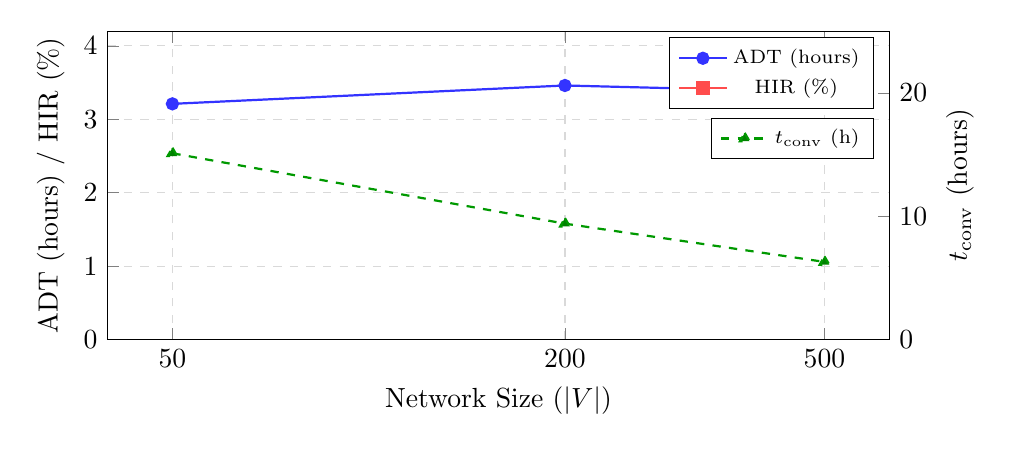
\begin{tikzpicture}
\begin{axis}[
    width=0.95\columnwidth,
    height=5.5cm,
    xlabel={Network Size ($|V|$)},
    ylabel={ADT (hours) / HIR (\%)},
    xmode=log,
    log basis x=10,
    xtick={50, 200, 500},
    xticklabels={50, 200, 500},
    ymin=0, ymax=4.2,
    axis y line*=left,
    legend style={at={(0.98,0.98)}, anchor=north east, font=\scriptsize},
    grid=major,
    grid style={dashed, gray!30},
]

% ADT
\addplot[thick, color=blue!80, mark=*, mark options={fill=blue!80}] coordinates {
    (50, 3.21) (200, 3.46) (500, 3.37)
};
\addlegendentry{ADT (hours)}

% HIR
\addplot[thick, color=red!70, mark=square*, mark options={fill=red!70}] coordinates {
    (50, 8.6) (200, 8.7) (500, 9.0)
};
\addlegendentry{HIR (\%)}

\end{axis}

\begin{axis}[
    width=0.95\columnwidth,
    height=5.5cm,
    xmode=log,
    log basis x=10,
    xtick=\empty,
    ylabel={$t_{\mathrm{conv}}$ (hours)},
    axis y line*=right,
    ymin=0, ymax=25,
    ylabel near ticks,
    legend style={at={(0.98,0.72)}, anchor=north east, font=\scriptsize},
]

% Convergence Time
\addplot[thick, color=green!60!black, mark=triangle*, mark options={fill=green!50!black}, dashed] coordinates {
    (50, 15.1) (200, 9.4) (500, 6.3)
};
\addlegendentry{$t_{\mathrm{conv}}$ (h)}

\end{axis}
\end{tikzpicture}
\caption{Scalability across network sizes in the released artifact. ADT and HIR remain stable from 50 to 500 nodes, while update time stays within real-time decision windows.}
\label{fig:scalability}
\end{figure}


% ================================================================
% Fig. 8: 军备竞赛动态 (Arms Race Dynamics)
% ================================================================
\begin{figure}[t]
\centering
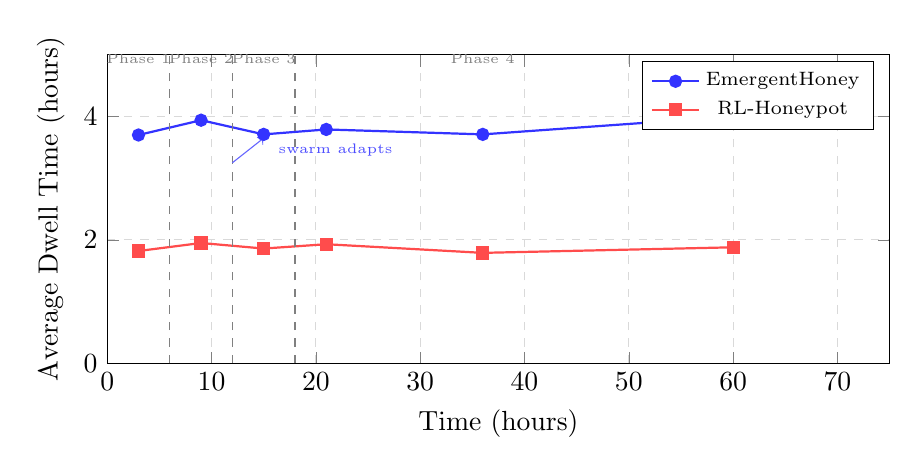
\begin{tikzpicture}
\begin{axis}[
    width=0.95\columnwidth,
    height=5.5cm,
    xlabel={Time (hours)},
    ylabel={Average Dwell Time (hours)},
    xmin=0, xmax=75,
    ymin=0, ymax=5,
    grid=major,
    grid style={dashed, gray!30},
    legend style={at={(0.98,0.98)}, anchor=north east, font=\scriptsize},
    mark size=2pt,
]

% EmergentHoney ADT
\addplot[thick, color=blue!80, mark=*, mark options={fill=blue!80}] coordinates {
    (3, 3.70) (9, 3.94) (15, 3.71) (21, 3.79) (36, 3.71) (60, 4.00)
};
\addlegendentry{EmergentHoney}

% RL-Honeypot ADT
\addplot[thick, color=red!70, mark=square*, mark options={fill=red!70}] coordinates {
    (3, 1.82) (9, 1.95) (15, 1.86) (21, 1.93) (36, 1.79) (60, 1.88)
};
\addlegendentry{RL-Honeypot}

% Phase annotations
\draw[thin, dashed, gray] (axis cs:6,0) -- (axis cs:6,5);
\draw[thin, dashed, gray] (axis cs:12,0) -- (axis cs:12,5);
\draw[thin, dashed, gray] (axis cs:18,0) -- (axis cs:18,5);

\node[font=\tiny, color=gray, anchor=south] at (axis cs:3, 4.7) {Phase 1};
\node[font=\tiny, color=gray, anchor=south] at (axis cs:9, 4.7) {Phase 2};
\node[font=\tiny, color=gray, anchor=south] at (axis cs:15, 4.7) {Phase 3};
\node[font=\tiny, color=gray, anchor=south] at (axis cs:36, 4.7) {Phase 4};

% Recovery annotation
\draw[->, thin, color=blue!60] (axis cs:12, 3.25) -- (axis cs:15, 3.65);
\node[font=\tiny, color=blue!70, anchor=west] at (axis cs:15.5, 3.45) {swarm adapts};

\end{axis}
\end{tikzpicture}
\caption{Arms race dynamics against an adaptive attacker in the canonical result bundle. EmergentHoney maintains roughly 2$\times$ the dwell time of the RL baseline throughout the full 72-hour horizon.}
\label{fig:arms_race}
\end{figure}


% ================================================================
% Fig. 2: 生物-网络同构映射示意 (Biological Isomorphism)
% ================================================================
\begin{figure*}[t]
\centering
\begin{tikzpicture}[
    ant/.style={circle, draw, fill=brown!30, minimum size=0.5cm, font=\tiny},
    hp/.style={circle, draw, fill=blue!20, minimum size=0.5cm, font=\tiny},
    food/.style={star, star points=5, draw, fill=yellow!50, minimum size=0.5cm, font=\tiny},
    attacker/.style={circle, draw, fill=red!20, minimum size=0.5cm, font=\tiny},
    trail/.style={thick, decorate, decoration={snake, amplitude=1pt, segment length=5pt}},
    pheromone/.style={thick, color=green!60!black},
]

% 左侧：蚂蚁觅食
\node[font=\small\bfseries] at (-4, 3.5) {Ant Colony Foraging};

% 巢穴
\node[rectangle, draw, fill=brown!10, minimum width=1cm, minimum height=0.6cm, font=\tiny] (nest) at (-6, 0) {Nest};

% 食物源
\node[food] (food1) at (-2.5, 2) {F1};
\node[food] (food2) at (-2, -1) {F2};

% 蚂蚁
\node[ant] (a1) at (-4.5, 1.2) {A1};
\node[ant] (a2) at (-3.5, 0.3) {A2};
\node[ant] (a3) at (-4, -0.8) {A3};

% 信息素路径
\draw[pheromone, line width=2pt, opacity=0.6] (nest) -- (a1) -- (food1);
\draw[pheromone, line width=1pt, opacity=0.3] (nest) -- (a3) -- (food2);
\draw[pheromone, line width=1.5pt, opacity=0.5] (nest) -- (a2);

% 右侧：EmergentHoney
\node[font=\small\bfseries] at (4, 3.5) {EmergentHoney};

% 真实网络
\node[rectangle, draw, fill=gray!10, minimum width=1cm, minimum height=0.6cm, font=\tiny] (real) at (2, 0) {Real\\Network};

% 蜜罐
\node[hp] (h1) at (5.5, 2) {$h_1$};
\node[hp] (h2) at (6, -1) {$h_2$};

% 攻击者
\node[attacker] (at1) at (3.5, 1.2) {Atk};

% 信息素路径
\draw[pheromone, line width=2pt, opacity=0.6] (real) -- (at1) -- (h1);
\draw[pheromone, line width=1pt, opacity=0.3] (real) -- (h2);

% 映射箭头
\draw[->, very thick, color=orange!70, dashed] (-1.5, 1.5) -- (1.5, 1.5);
\node[font=\scriptsize\itshape, color=orange!70] at (0, 2) {Isomorphism};
\draw[->, very thick, color=orange!70, dashed] (-1.5, -0.5) -- (1.5, -0.5);

% 映射标签
\node[font=\tiny, anchor=west] at (-1.2, 1.0) {Ant $\leftrightarrow$ Honeypot};
\node[font=\tiny, anchor=west] at (-1.2, 0.3) {Pheromone $\leftrightarrow$ Attack signal};
\node[font=\tiny, anchor=west] at (-1.2, -0.3) {Food $\leftrightarrow$ Attacker engagement};
\node[font=\tiny, anchor=west] at (-1.2, -1.0) {Evaporation $\leftrightarrow$ Strategy retirement};

\end{tikzpicture}
\caption{Biological--cyber isomorphism between ant colony foraging and EmergentHoney. Ants map to honeypots, pheromone trails to attack signals, food sources to attacker engagement, and evaporation to strategy retirement.}
\label{fig:isomorphism}
\end{figure*}
 引入
% ================================================================

% ================================================================
% Fig. 1: 系统架构图 (System Architecture Overview)
% ================================================================
\begin{figure*}[t]
\centering
\begin{tikzpicture}[
    node distance=1.2cm and 1.8cm,
    block/.style={rectangle, draw, rounded corners, fill=blue!8, minimum width=2.8cm, minimum height=1cm, align=center, font=\small},
    bigblock/.style={rectangle, draw, rounded corners, fill=orange!8, minimum width=3.2cm, minimum height=1cm, align=center, font=\small},
    datablock/.style={rectangle, draw, rounded corners, fill=green!8, minimum width=2.5cm, minimum height=0.8cm, align=center, font=\small},
    arrow/.style={->, thick, >=stealth},
    dasharrow/.style={->, thick, dashed, >=stealth, color=red!60},
    label/.style={font=\footnotesize\itshape, color=gray}
]

% 第一层：攻击者
\node[block, fill=red!12] (attacker) {Attacker\\(L1/L2/L3)};

% 第二层：SDN网络层
\node[bigblock, below=1.5cm of attacker] (sdn) {SDN Network Layer\\(OpenFlow / Mininet)};

% 第三层：蜜罐群
\node[block, below left=1.5cm and 1cm of sdn] (hp1) {Honeypot $h_1$\\(SSH/Cowrie)};
\node[block, below=1.5cm of sdn] (hp2) {Honeypot $h_2$\\(HTTP/Snare)};
\node[block, below right=1.5cm and 1cm of sdn] (hp3) {Honeypot $h_n$\\(MySQL/OpenCanary)};
\node[font=\large] at ($(hp2)!0.5!(hp3) + (0, 0.0)$) {$\cdots$};

% 第四层：核心模块
\node[bigblock, fill=yellow!15, below=1.5cm of hp1] (pheromone) {Pheromone Engine\\$\tau_{ij}(t{+}1) = (1{-}\rho)\tau_{ij}(t) + \sum_k \Delta\tau_{ij}^k$};
\node[bigblock, fill=purple!10, below=1.5cm of hp3] (llm) {LLM Phenotype\\Generator\\(GPT-4o / Llama-3)};
\node[bigblock, fill=cyan!10, below=2.8cm of hp2] (reverse) {Reverse ACO\\Attacker Model};

% 连线
\draw[arrow] (attacker) -- node[right, label] {probes / exploits} (sdn);
\draw[arrow] (sdn) -- (hp1);
\draw[arrow] (sdn) -- (hp2);
\draw[arrow] (sdn) -- (hp3);

\draw[arrow, color=blue!70] (hp1) -- node[left, label] {interaction\\logs} (pheromone);
\draw[arrow, color=blue!70] (hp2) -- (pheromone);
\draw[dasharrow] (hp1) -- (llm);
\draw[arrow, color=blue!70] (hp3) -- (llm);

\draw[arrow, color=orange!80] (pheromone) -- node[below, label] {deploy/migrate/mutate} (reverse);
\draw[arrow, color=purple!70] (llm) -- node[below, label] {phenotype content} (reverse);

\draw[arrow, color=green!60!black, bend left=30] (pheromone.north) to node[left, label] {self-org\\commands} (sdn.south west);
\draw[arrow, color=green!60!black, bend right=30] (reverse.north) to node[right, label] {predictive\\placement} (sdn.south east);

% 外框
\node[draw, dashed, thick, rounded corners, fit=(hp1)(hp2)(hp3)(pheromone)(llm)(reverse), inner sep=10pt, label={[font=\small\bfseries]above:EmergentHoney Framework}] {};

\end{tikzpicture}
\caption{System architecture of EmergentHoney. Attacker interactions with honeypots generate pheromone deposits that drive self-organization (proliferation, migration, mutation). The LLM phenotype generator creates context-aware deception content. The Reverse ACO module predicts attacker targets for preemptive deployment.}
\label{fig:architecture}
\end{figure*}


% ================================================================
% Fig. 4: 欺骗效果对比柱状图 (ADT Comparison Bar Chart)
% ================================================================
\begin{figure}[t]
\centering
\begin{tikzpicture}
\begin{axis}[
    ybar,
    bar width=10pt,
    width=0.95\columnwidth,
    height=6cm,
    ylabel={Average Dwell Time (hours)},
    symbolic x coords={Static, Rand-Dyn, RL-HP, Game-Th, GAN-HP, LLM-St, EH},
    xtick=data,
    x tick label style={rotate=30, anchor=east, font=\footnotesize},
    ymin=0, ymax=4.2,
    nodes near coords,
    nodes near coords style={font=\tiny, above},
    legend style={at={(0.02,0.98)}, anchor=north west, font=\scriptsize},
    error bars/.cd, y dir=both, y explicit,
]
\addplot+[fill=gray!40, draw=gray!60] coordinates {
    (Static, 1.57) +- (0, 0.11)
    (Rand-Dyn, 1.55) +- (0, 0.10)
    (RL-HP, 1.66) +- (0, 0.10)
    (Game-Th, 1.59) +- (0, 0.10)
    (GAN-HP, 1.76) +- (0, 0.11)
    (LLM-St, 2.43) +- (0, 0.12)
    (EH, 3.24) +- (0, 0.16)
};
\end{axis}
\end{tikzpicture}
\caption{Average Dwell Time comparison across all methods on the medium network. EmergentHoney (EH) achieves 3.24 hours, outperforming the best adaptive baseline (RL-Honeypot) by 96\%.}
\label{fig:adt_comparison}
\end{figure}


% ================================================================
% Fig. 5: DEI 随时间变化曲线 (DEI Over Time)
% ================================================================
\begin{figure}[t]
\centering
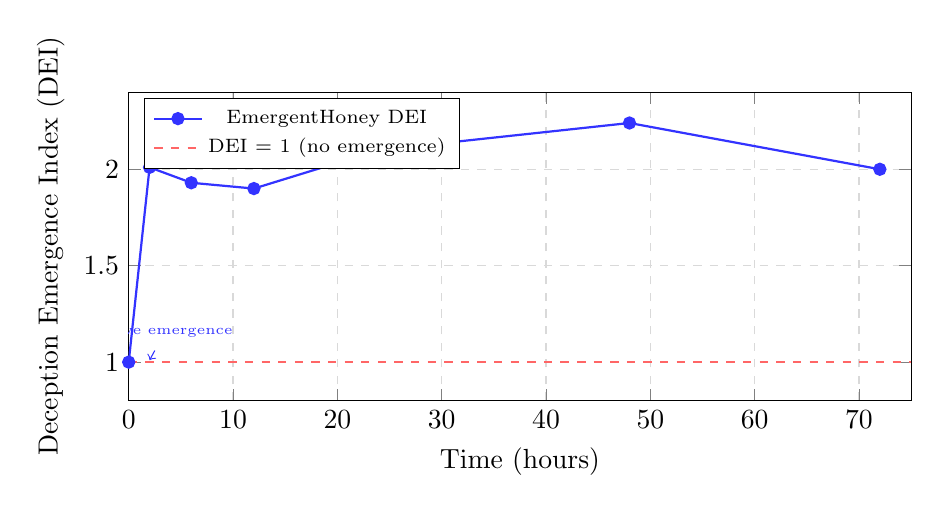
\begin{tikzpicture}
\begin{axis}[
    width=0.95\columnwidth,
    height=5.5cm,
    xlabel={Time (hours)},
    ylabel={Deception Emergence Index (DEI)},
    xmin=0, xmax=75,
    ymin=0.8, ymax=2.4,
    grid=major,
    grid style={dashed, gray!30},
    legend style={at={(0.02,0.98)}, anchor=north west, font=\scriptsize},
    mark size=2pt,
]

% DEI 曲线
\addplot[thick, color=blue!80, mark=*, mark options={fill=blue!80}] coordinates {
    (0, 1.00) (2, 2.01) (6, 1.93) (12, 1.90) (24, 2.10) (48, 2.24) (72, 2.00)
};
\addlegendentry{EmergentHoney DEI}

% DEI = 1 参考线
\addplot[dashed, thick, color=red!60, domain=0:75] {1.0};
\addlegendentry{DEI = 1 (no emergence)}

\node[font=\tiny, color=blue!80, anchor=south] at (axis cs:2.5, 1.08) {positive emergence};
\draw[->, thin, color=blue!80] (axis cs:2.5, 1.06) -- (axis cs:2.0, 1.01);

\end{axis}
\end{tikzpicture}
\caption{DEI evolution over time in the canonical result bundle. The swarm rapidly enters the positive-emergence regime and stabilizes near DEI $\approx 2.0$.}
\label{fig:dei_curve}
\end{figure}


% ================================================================
% Fig. 6: 消融实验雷达图 (Ablation Radar Chart)
% ================================================================
\begin{figure}[t]
\centering
\begin{tikzpicture}
\begin{polaraxis}[
    width=0.85\columnwidth,
    height=0.85\columnwidth,
    xtick={0, 45, 90, 135, 180, 225, 270, 315},
    xticklabels={ADT, TIC, DEI, {1-HIR}, {ADT}, {TIC}, {DEI}, {1-HIR}},
    xticklabel style={font=\tiny},
    ymin=0, ymax=1.1,
    ytick={0.2, 0.4, 0.6, 0.8, 1.0},
    yticklabels={0.2, 0.4, 0.6, 0.8, 1.0},
    yticklabel style={font=\tiny},
    legend style={at={(1.3,1.0)}, anchor=north, font=\tiny},
]

% Full EmergentHoney (归一化到[0,1])
\addplot[thick, color=blue!80, fill=blue!15, mark=*, mark size=1.5pt] coordinates {
    (0, 1.0) (90, 1.0) (180, 1.0) (270, 1.0) (360, 1.0)
};
\addlegendentry{Full}

% w/o Pheromone
\addplot[thick, color=red!70, fill=red!5, mark=square*, mark size=1.5pt] coordinates {
    (0, 0.45) (90, 0.43) (180, 0.61) (270, 0.52) (360, 0.45)
};
\addlegendentry{w/o Pheromone}

% w/o LLM
\addplot[thick, color=green!60!black, fill=green!5, mark=triangle*, mark size=1.5pt] coordinates {
    (0, 0.72) (90, 0.72) (180, 0.94) (270, 0.84) (360, 0.72)
};
\addlegendentry{w/o LLM}

\end{polaraxis}
\end{tikzpicture}
\caption{Ablation study radar chart (normalized). The full EmergentHoney system forms the outer boundary. Removing the pheromone mechanism causes the most severe degradation.}
\label{fig:ablation_radar}
\end{figure}


% ================================================================
% Fig. 7: 可扩展性 (Scalability - Dual Y-Axis)
% ================================================================
\begin{figure}[t]
\centering
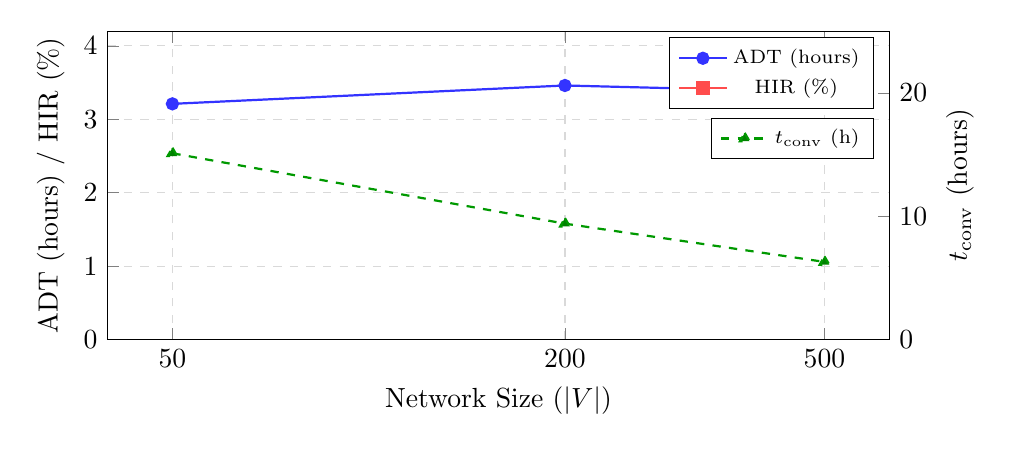
\begin{tikzpicture}
\begin{axis}[
    width=0.95\columnwidth,
    height=5.5cm,
    xlabel={Network Size ($|V|$)},
    ylabel={ADT (hours) / HIR (\%)},
    xmode=log,
    log basis x=10,
    xtick={50, 200, 500},
    xticklabels={50, 200, 500},
    ymin=0, ymax=4.2,
    axis y line*=left,
    legend style={at={(0.98,0.98)}, anchor=north east, font=\scriptsize},
    grid=major,
    grid style={dashed, gray!30},
]

% ADT
\addplot[thick, color=blue!80, mark=*, mark options={fill=blue!80}] coordinates {
    (50, 3.21) (200, 3.46) (500, 3.37)
};
\addlegendentry{ADT (hours)}

% HIR
\addplot[thick, color=red!70, mark=square*, mark options={fill=red!70}] coordinates {
    (50, 8.6) (200, 8.7) (500, 9.0)
};
\addlegendentry{HIR (\%)}

\end{axis}

\begin{axis}[
    width=0.95\columnwidth,
    height=5.5cm,
    xmode=log,
    log basis x=10,
    xtick=\empty,
    ylabel={$t_{\mathrm{conv}}$ (hours)},
    axis y line*=right,
    ymin=0, ymax=25,
    ylabel near ticks,
    legend style={at={(0.98,0.72)}, anchor=north east, font=\scriptsize},
]

% Convergence Time
\addplot[thick, color=green!60!black, mark=triangle*, mark options={fill=green!50!black}, dashed] coordinates {
    (50, 15.1) (200, 9.4) (500, 6.3)
};
\addlegendentry{$t_{\mathrm{conv}}$ (h)}

\end{axis}
\end{tikzpicture}
\caption{Scalability across network sizes in the released artifact. ADT and HIR remain stable from 50 to 500 nodes, while update time stays within real-time decision windows.}
\label{fig:scalability}
\end{figure}


% ================================================================
% Fig. 8: 军备竞赛动态 (Arms Race Dynamics)
% ================================================================
\begin{figure}[t]
\centering
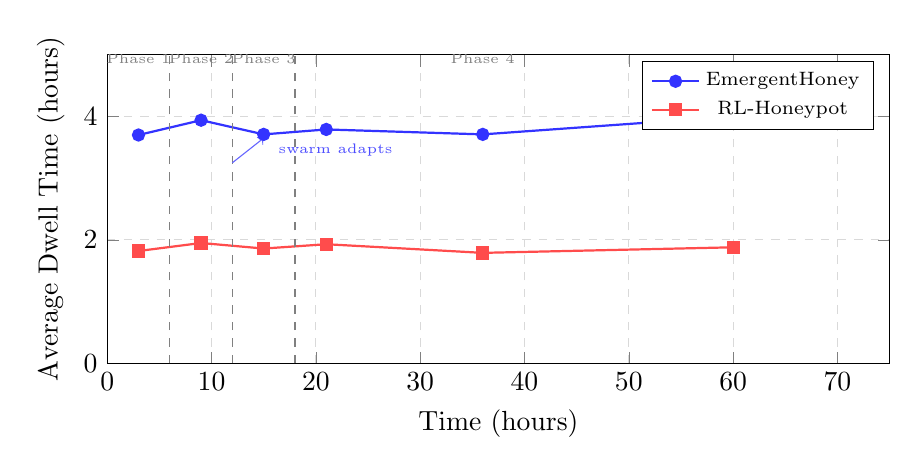
\begin{tikzpicture}
\begin{axis}[
    width=0.95\columnwidth,
    height=5.5cm,
    xlabel={Time (hours)},
    ylabel={Average Dwell Time (hours)},
    xmin=0, xmax=75,
    ymin=0, ymax=5,
    grid=major,
    grid style={dashed, gray!30},
    legend style={at={(0.98,0.98)}, anchor=north east, font=\scriptsize},
    mark size=2pt,
]

% EmergentHoney ADT
\addplot[thick, color=blue!80, mark=*, mark options={fill=blue!80}] coordinates {
    (3, 3.70) (9, 3.94) (15, 3.71) (21, 3.79) (36, 3.71) (60, 4.00)
};
\addlegendentry{EmergentHoney}

% RL-Honeypot ADT
\addplot[thick, color=red!70, mark=square*, mark options={fill=red!70}] coordinates {
    (3, 1.82) (9, 1.95) (15, 1.86) (21, 1.93) (36, 1.79) (60, 1.88)
};
\addlegendentry{RL-Honeypot}

% Phase annotations
\draw[thin, dashed, gray] (axis cs:6,0) -- (axis cs:6,5);
\draw[thin, dashed, gray] (axis cs:12,0) -- (axis cs:12,5);
\draw[thin, dashed, gray] (axis cs:18,0) -- (axis cs:18,5);

\node[font=\tiny, color=gray, anchor=south] at (axis cs:3, 4.7) {Phase 1};
\node[font=\tiny, color=gray, anchor=south] at (axis cs:9, 4.7) {Phase 2};
\node[font=\tiny, color=gray, anchor=south] at (axis cs:15, 4.7) {Phase 3};
\node[font=\tiny, color=gray, anchor=south] at (axis cs:36, 4.7) {Phase 4};

% Recovery annotation
\draw[->, thin, color=blue!60] (axis cs:12, 3.25) -- (axis cs:15, 3.65);
\node[font=\tiny, color=blue!70, anchor=west] at (axis cs:15.5, 3.45) {swarm adapts};

\end{axis}
\end{tikzpicture}
\caption{Arms race dynamics against an adaptive attacker in the canonical result bundle. EmergentHoney maintains roughly 2$\times$ the dwell time of the RL baseline throughout the full 72-hour horizon.}
\label{fig:arms_race}
\end{figure}


% ================================================================
% Fig. 2: 生物-网络同构映射示意 (Biological Isomorphism)
% ================================================================
\begin{figure*}[t]
\centering
\begin{tikzpicture}[
    ant/.style={circle, draw, fill=brown!30, minimum size=0.5cm, font=\tiny},
    hp/.style={circle, draw, fill=blue!20, minimum size=0.5cm, font=\tiny},
    food/.style={star, star points=5, draw, fill=yellow!50, minimum size=0.5cm, font=\tiny},
    attacker/.style={circle, draw, fill=red!20, minimum size=0.5cm, font=\tiny},
    trail/.style={thick, decorate, decoration={snake, amplitude=1pt, segment length=5pt}},
    pheromone/.style={thick, color=green!60!black},
]

% 左侧：蚂蚁觅食
\node[font=\small\bfseries] at (-4, 3.5) {Ant Colony Foraging};

% 巢穴
\node[rectangle, draw, fill=brown!10, minimum width=1cm, minimum height=0.6cm, font=\tiny] (nest) at (-6, 0) {Nest};

% 食物源
\node[food] (food1) at (-2.5, 2) {F1};
\node[food] (food2) at (-2, -1) {F2};

% 蚂蚁
\node[ant] (a1) at (-4.5, 1.2) {A1};
\node[ant] (a2) at (-3.5, 0.3) {A2};
\node[ant] (a3) at (-4, -0.8) {A3};

% 信息素路径
\draw[pheromone, line width=2pt, opacity=0.6] (nest) -- (a1) -- (food1);
\draw[pheromone, line width=1pt, opacity=0.3] (nest) -- (a3) -- (food2);
\draw[pheromone, line width=1.5pt, opacity=0.5] (nest) -- (a2);

% 右侧：EmergentHoney
\node[font=\small\bfseries] at (4, 3.5) {EmergentHoney};

% 真实网络
\node[rectangle, draw, fill=gray!10, minimum width=1cm, minimum height=0.6cm, font=\tiny] (real) at (2, 0) {Real\\Network};

% 蜜罐
\node[hp] (h1) at (5.5, 2) {$h_1$};
\node[hp] (h2) at (6, -1) {$h_2$};

% 攻击者
\node[attacker] (at1) at (3.5, 1.2) {Atk};

% 信息素路径
\draw[pheromone, line width=2pt, opacity=0.6] (real) -- (at1) -- (h1);
\draw[pheromone, line width=1pt, opacity=0.3] (real) -- (h2);

% 映射箭头
\draw[->, very thick, color=orange!70, dashed] (-1.5, 1.5) -- (1.5, 1.5);
\node[font=\scriptsize\itshape, color=orange!70] at (0, 2) {Isomorphism};
\draw[->, very thick, color=orange!70, dashed] (-1.5, -0.5) -- (1.5, -0.5);

% 映射标签
\node[font=\tiny, anchor=west] at (-1.2, 1.0) {Ant $\leftrightarrow$ Honeypot};
\node[font=\tiny, anchor=west] at (-1.2, 0.3) {Pheromone $\leftrightarrow$ Attack signal};
\node[font=\tiny, anchor=west] at (-1.2, -0.3) {Food $\leftrightarrow$ Attacker engagement};
\node[font=\tiny, anchor=west] at (-1.2, -1.0) {Evaporation $\leftrightarrow$ Strategy retirement};

\end{tikzpicture}
\caption{Biological--cyber isomorphism between ant colony foraging and EmergentHoney. Ants map to honeypots, pheromone trails to attack signals, food sources to attacker engagement, and evaporation to strategy retirement.}
\label{fig:isomorphism}
\end{figure*}
 引入
% ================================================================

% ================================================================
% Fig. 1: 系统架构图 (System Architecture Overview)
% ================================================================
\begin{figure*}[t]
\centering
\begin{tikzpicture}[
    node distance=1.2cm and 1.8cm,
    block/.style={rectangle, draw, rounded corners, fill=blue!8, minimum width=2.8cm, minimum height=1cm, align=center, font=\small},
    bigblock/.style={rectangle, draw, rounded corners, fill=orange!8, minimum width=3.2cm, minimum height=1cm, align=center, font=\small},
    datablock/.style={rectangle, draw, rounded corners, fill=green!8, minimum width=2.5cm, minimum height=0.8cm, align=center, font=\small},
    arrow/.style={->, thick, >=stealth},
    dasharrow/.style={->, thick, dashed, >=stealth, color=red!60},
    label/.style={font=\footnotesize\itshape, color=gray}
]

% 第一层：攻击者
\node[block, fill=red!12] (attacker) {Attacker\\(L1/L2/L3)};

% 第二层：SDN网络层
\node[bigblock, below=1.5cm of attacker] (sdn) {SDN Network Layer\\(OpenFlow / Mininet)};

% 第三层：蜜罐群
\node[block, below left=1.5cm and 1cm of sdn] (hp1) {Honeypot $h_1$\\(SSH/Cowrie)};
\node[block, below=1.5cm of sdn] (hp2) {Honeypot $h_2$\\(HTTP/Snare)};
\node[block, below right=1.5cm and 1cm of sdn] (hp3) {Honeypot $h_n$\\(MySQL/OpenCanary)};
\node[font=\large] at ($(hp2)!0.5!(hp3) + (0, 0.0)$) {$\cdots$};

% 第四层：核心模块
\node[bigblock, fill=yellow!15, below=1.5cm of hp1] (pheromone) {Pheromone Engine\\$\tau_{ij}(t{+}1) = (1{-}\rho)\tau_{ij}(t) + \sum_k \Delta\tau_{ij}^k$};
\node[bigblock, fill=purple!10, below=1.5cm of hp3] (llm) {LLM Phenotype\\Generator\\(GPT-4o / Llama-3)};
\node[bigblock, fill=cyan!10, below=2.8cm of hp2] (reverse) {Reverse ACO\\Attacker Model};

% 连线
\draw[arrow] (attacker) -- node[right, label] {probes / exploits} (sdn);
\draw[arrow] (sdn) -- (hp1);
\draw[arrow] (sdn) -- (hp2);
\draw[arrow] (sdn) -- (hp3);

\draw[arrow, color=blue!70] (hp1) -- node[left, label] {interaction\\logs} (pheromone);
\draw[arrow, color=blue!70] (hp2) -- (pheromone);
\draw[dasharrow] (hp1) -- (llm);
\draw[arrow, color=blue!70] (hp3) -- (llm);

\draw[arrow, color=orange!80] (pheromone) -- node[below, label] {deploy/migrate/mutate} (reverse);
\draw[arrow, color=purple!70] (llm) -- node[below, label] {phenotype content} (reverse);

\draw[arrow, color=green!60!black, bend left=30] (pheromone.north) to node[left, label] {self-org\\commands} (sdn.south west);
\draw[arrow, color=green!60!black, bend right=30] (reverse.north) to node[right, label] {predictive\\placement} (sdn.south east);

% 外框
\node[draw, dashed, thick, rounded corners, fit=(hp1)(hp2)(hp3)(pheromone)(llm)(reverse), inner sep=10pt, label={[font=\small\bfseries]above:EmergentHoney Framework}] {};

\end{tikzpicture}
\caption{System architecture of EmergentHoney. Attacker interactions with honeypots generate pheromone deposits that drive self-organization (proliferation, migration, mutation). The LLM phenotype generator creates context-aware deception content. The Reverse ACO module predicts attacker targets for preemptive deployment.}
\label{fig:architecture}
\end{figure*}


% ================================================================
% Fig. 4: 欺骗效果对比柱状图 (ADT Comparison Bar Chart)
% ================================================================
\begin{figure}[t]
\centering
\begin{tikzpicture}
\begin{axis}[
    ybar,
    bar width=10pt,
    width=0.95\columnwidth,
    height=6cm,
    ylabel={Average Dwell Time (hours)},
    symbolic x coords={Static, Rand-Dyn, RL-HP, Game-Th, GAN-HP, LLM-St, EH},
    xtick=data,
    x tick label style={rotate=30, anchor=east, font=\footnotesize},
    ymin=0, ymax=4.2,
    nodes near coords,
    nodes near coords style={font=\tiny, above},
    legend style={at={(0.02,0.98)}, anchor=north west, font=\scriptsize},
    error bars/.cd, y dir=both, y explicit,
]
\addplot+[fill=gray!40, draw=gray!60] coordinates {
    (Static, 1.57) +- (0, 0.11)
    (Rand-Dyn, 1.55) +- (0, 0.10)
    (RL-HP, 1.66) +- (0, 0.10)
    (Game-Th, 1.59) +- (0, 0.10)
    (GAN-HP, 1.76) +- (0, 0.11)
    (LLM-St, 2.43) +- (0, 0.12)
    (EH, 3.24) +- (0, 0.16)
};
\end{axis}
\end{tikzpicture}
\caption{Average Dwell Time comparison across all methods on the medium network. EmergentHoney (EH) achieves 3.24 hours, outperforming the best adaptive baseline (RL-Honeypot) by 96\%.}
\label{fig:adt_comparison}
\end{figure}


% ================================================================
% Fig. 5: DEI 随时间变化曲线 (DEI Over Time)
% ================================================================
\begin{figure}[t]
\centering
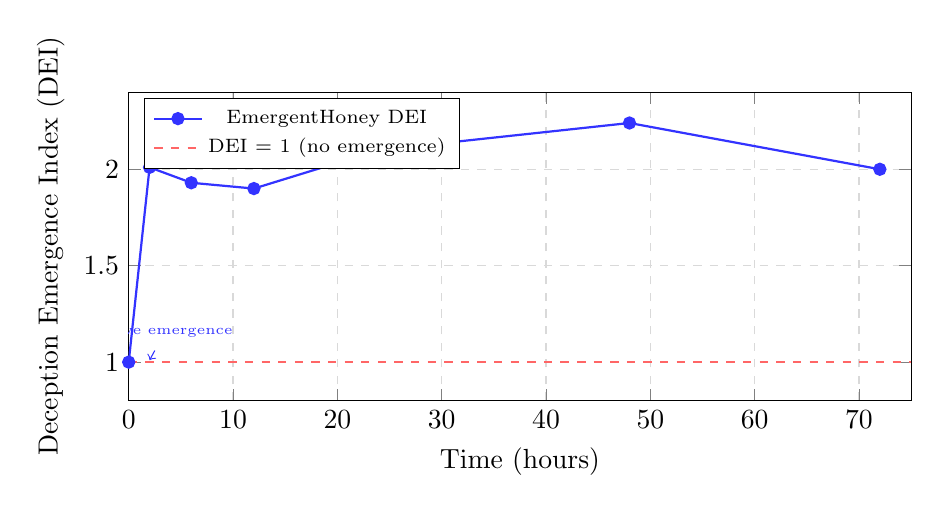
\begin{tikzpicture}
\begin{axis}[
    width=0.95\columnwidth,
    height=5.5cm,
    xlabel={Time (hours)},
    ylabel={Deception Emergence Index (DEI)},
    xmin=0, xmax=75,
    ymin=0.8, ymax=2.4,
    grid=major,
    grid style={dashed, gray!30},
    legend style={at={(0.02,0.98)}, anchor=north west, font=\scriptsize},
    mark size=2pt,
]

% DEI 曲线
\addplot[thick, color=blue!80, mark=*, mark options={fill=blue!80}] coordinates {
    (0, 1.00) (2, 2.01) (6, 1.93) (12, 1.90) (24, 2.10) (48, 2.24) (72, 2.00)
};
\addlegendentry{EmergentHoney DEI}

% DEI = 1 参考线
\addplot[dashed, thick, color=red!60, domain=0:75] {1.0};
\addlegendentry{DEI = 1 (no emergence)}

\node[font=\tiny, color=blue!80, anchor=south] at (axis cs:2.5, 1.08) {positive emergence};
\draw[->, thin, color=blue!80] (axis cs:2.5, 1.06) -- (axis cs:2.0, 1.01);

\end{axis}
\end{tikzpicture}
\caption{DEI evolution over time in the canonical result bundle. The swarm rapidly enters the positive-emergence regime and stabilizes near DEI $\approx 2.0$.}
\label{fig:dei_curve}
\end{figure}


% ================================================================
% Fig. 6: 消融实验雷达图 (Ablation Radar Chart)
% ================================================================
\begin{figure}[t]
\centering
\begin{tikzpicture}
\begin{polaraxis}[
    width=0.85\columnwidth,
    height=0.85\columnwidth,
    xtick={0, 45, 90, 135, 180, 225, 270, 315},
    xticklabels={ADT, TIC, DEI, {1-HIR}, {ADT}, {TIC}, {DEI}, {1-HIR}},
    xticklabel style={font=\tiny},
    ymin=0, ymax=1.1,
    ytick={0.2, 0.4, 0.6, 0.8, 1.0},
    yticklabels={0.2, 0.4, 0.6, 0.8, 1.0},
    yticklabel style={font=\tiny},
    legend style={at={(1.3,1.0)}, anchor=north, font=\tiny},
]

% Full EmergentHoney (归一化到[0,1])
\addplot[thick, color=blue!80, fill=blue!15, mark=*, mark size=1.5pt] coordinates {
    (0, 1.0) (90, 1.0) (180, 1.0) (270, 1.0) (360, 1.0)
};
\addlegendentry{Full}

% w/o Pheromone
\addplot[thick, color=red!70, fill=red!5, mark=square*, mark size=1.5pt] coordinates {
    (0, 0.45) (90, 0.43) (180, 0.61) (270, 0.52) (360, 0.45)
};
\addlegendentry{w/o Pheromone}

% w/o LLM
\addplot[thick, color=green!60!black, fill=green!5, mark=triangle*, mark size=1.5pt] coordinates {
    (0, 0.72) (90, 0.72) (180, 0.94) (270, 0.84) (360, 0.72)
};
\addlegendentry{w/o LLM}

\end{polaraxis}
\end{tikzpicture}
\caption{Ablation study radar chart (normalized). The full EmergentHoney system forms the outer boundary. Removing the pheromone mechanism causes the most severe degradation.}
\label{fig:ablation_radar}
\end{figure}


% ================================================================
% Fig. 7: 可扩展性 (Scalability - Dual Y-Axis)
% ================================================================
\begin{figure}[t]
\centering
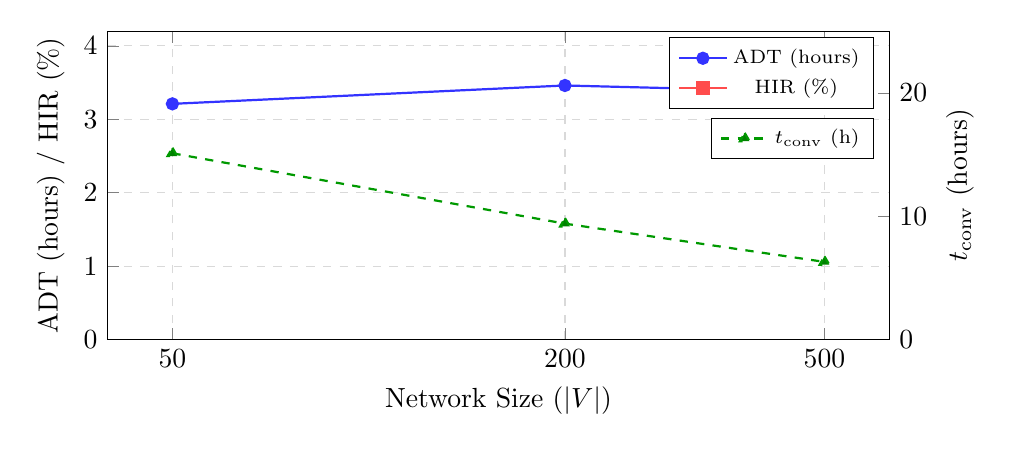
\begin{tikzpicture}
\begin{axis}[
    width=0.95\columnwidth,
    height=5.5cm,
    xlabel={Network Size ($|V|$)},
    ylabel={ADT (hours) / HIR (\%)},
    xmode=log,
    log basis x=10,
    xtick={50, 200, 500},
    xticklabels={50, 200, 500},
    ymin=0, ymax=4.2,
    axis y line*=left,
    legend style={at={(0.98,0.98)}, anchor=north east, font=\scriptsize},
    grid=major,
    grid style={dashed, gray!30},
]

% ADT
\addplot[thick, color=blue!80, mark=*, mark options={fill=blue!80}] coordinates {
    (50, 3.21) (200, 3.46) (500, 3.37)
};
\addlegendentry{ADT (hours)}

% HIR
\addplot[thick, color=red!70, mark=square*, mark options={fill=red!70}] coordinates {
    (50, 8.6) (200, 8.7) (500, 9.0)
};
\addlegendentry{HIR (\%)}

\end{axis}

\begin{axis}[
    width=0.95\columnwidth,
    height=5.5cm,
    xmode=log,
    log basis x=10,
    xtick=\empty,
    ylabel={$t_{\mathrm{conv}}$ (hours)},
    axis y line*=right,
    ymin=0, ymax=25,
    ylabel near ticks,
    legend style={at={(0.98,0.72)}, anchor=north east, font=\scriptsize},
]

% Convergence Time
\addplot[thick, color=green!60!black, mark=triangle*, mark options={fill=green!50!black}, dashed] coordinates {
    (50, 15.1) (200, 9.4) (500, 6.3)
};
\addlegendentry{$t_{\mathrm{conv}}$ (h)}

\end{axis}
\end{tikzpicture}
\caption{Scalability across network sizes in the released artifact. ADT and HIR remain stable from 50 to 500 nodes, while update time stays within real-time decision windows.}
\label{fig:scalability}
\end{figure}


% ================================================================
% Fig. 8: 军备竞赛动态 (Arms Race Dynamics)
% ================================================================
\begin{figure}[t]
\centering
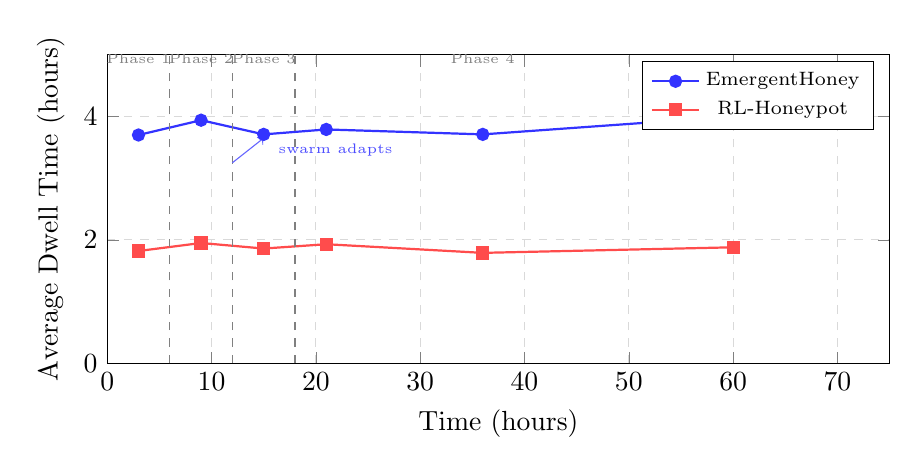
\begin{tikzpicture}
\begin{axis}[
    width=0.95\columnwidth,
    height=5.5cm,
    xlabel={Time (hours)},
    ylabel={Average Dwell Time (hours)},
    xmin=0, xmax=75,
    ymin=0, ymax=5,
    grid=major,
    grid style={dashed, gray!30},
    legend style={at={(0.98,0.98)}, anchor=north east, font=\scriptsize},
    mark size=2pt,
]

% EmergentHoney ADT
\addplot[thick, color=blue!80, mark=*, mark options={fill=blue!80}] coordinates {
    (3, 3.70) (9, 3.94) (15, 3.71) (21, 3.79) (36, 3.71) (60, 4.00)
};
\addlegendentry{EmergentHoney}

% RL-Honeypot ADT
\addplot[thick, color=red!70, mark=square*, mark options={fill=red!70}] coordinates {
    (3, 1.82) (9, 1.95) (15, 1.86) (21, 1.93) (36, 1.79) (60, 1.88)
};
\addlegendentry{RL-Honeypot}

% Phase annotations
\draw[thin, dashed, gray] (axis cs:6,0) -- (axis cs:6,5);
\draw[thin, dashed, gray] (axis cs:12,0) -- (axis cs:12,5);
\draw[thin, dashed, gray] (axis cs:18,0) -- (axis cs:18,5);

\node[font=\tiny, color=gray, anchor=south] at (axis cs:3, 4.7) {Phase 1};
\node[font=\tiny, color=gray, anchor=south] at (axis cs:9, 4.7) {Phase 2};
\node[font=\tiny, color=gray, anchor=south] at (axis cs:15, 4.7) {Phase 3};
\node[font=\tiny, color=gray, anchor=south] at (axis cs:36, 4.7) {Phase 4};

% Recovery annotation
\draw[->, thin, color=blue!60] (axis cs:12, 3.25) -- (axis cs:15, 3.65);
\node[font=\tiny, color=blue!70, anchor=west] at (axis cs:15.5, 3.45) {swarm adapts};

\end{axis}
\end{tikzpicture}
\caption{Arms race dynamics against an adaptive attacker in the canonical result bundle. EmergentHoney maintains roughly 2$\times$ the dwell time of the RL baseline throughout the full 72-hour horizon.}
\label{fig:arms_race}
\end{figure}


% ================================================================
% Fig. 2: 生物-网络同构映射示意 (Biological Isomorphism)
% ================================================================
\begin{figure*}[t]
\centering
\begin{tikzpicture}[
    ant/.style={circle, draw, fill=brown!30, minimum size=0.5cm, font=\tiny},
    hp/.style={circle, draw, fill=blue!20, minimum size=0.5cm, font=\tiny},
    food/.style={star, star points=5, draw, fill=yellow!50, minimum size=0.5cm, font=\tiny},
    attacker/.style={circle, draw, fill=red!20, minimum size=0.5cm, font=\tiny},
    trail/.style={thick, decorate, decoration={snake, amplitude=1pt, segment length=5pt}},
    pheromone/.style={thick, color=green!60!black},
]

% 左侧：蚂蚁觅食
\node[font=\small\bfseries] at (-4, 3.5) {Ant Colony Foraging};

% 巢穴
\node[rectangle, draw, fill=brown!10, minimum width=1cm, minimum height=0.6cm, font=\tiny] (nest) at (-6, 0) {Nest};

% 食物源
\node[food] (food1) at (-2.5, 2) {F1};
\node[food] (food2) at (-2, -1) {F2};

% 蚂蚁
\node[ant] (a1) at (-4.5, 1.2) {A1};
\node[ant] (a2) at (-3.5, 0.3) {A2};
\node[ant] (a3) at (-4, -0.8) {A3};

% 信息素路径
\draw[pheromone, line width=2pt, opacity=0.6] (nest) -- (a1) -- (food1);
\draw[pheromone, line width=1pt, opacity=0.3] (nest) -- (a3) -- (food2);
\draw[pheromone, line width=1.5pt, opacity=0.5] (nest) -- (a2);

% 右侧：EmergentHoney
\node[font=\small\bfseries] at (4, 3.5) {EmergentHoney};

% 真实网络
\node[rectangle, draw, fill=gray!10, minimum width=1cm, minimum height=0.6cm, font=\tiny] (real) at (2, 0) {Real\\Network};

% 蜜罐
\node[hp] (h1) at (5.5, 2) {$h_1$};
\node[hp] (h2) at (6, -1) {$h_2$};

% 攻击者
\node[attacker] (at1) at (3.5, 1.2) {Atk};

% 信息素路径
\draw[pheromone, line width=2pt, opacity=0.6] (real) -- (at1) -- (h1);
\draw[pheromone, line width=1pt, opacity=0.3] (real) -- (h2);

% 映射箭头
\draw[->, very thick, color=orange!70, dashed] (-1.5, 1.5) -- (1.5, 1.5);
\node[font=\scriptsize\itshape, color=orange!70] at (0, 2) {Isomorphism};
\draw[->, very thick, color=orange!70, dashed] (-1.5, -0.5) -- (1.5, -0.5);

% 映射标签
\node[font=\tiny, anchor=west] at (-1.2, 1.0) {Ant $\leftrightarrow$ Honeypot};
\node[font=\tiny, anchor=west] at (-1.2, 0.3) {Pheromone $\leftrightarrow$ Attack signal};
\node[font=\tiny, anchor=west] at (-1.2, -0.3) {Food $\leftrightarrow$ Attacker engagement};
\node[font=\tiny, anchor=west] at (-1.2, -1.0) {Evaporation $\leftrightarrow$ Strategy retirement};

\end{tikzpicture}
\caption{Biological--cyber isomorphism between ant colony foraging and EmergentHoney. Ants map to honeypots, pheromone trails to attack signals, food sources to attacker engagement, and evaporation to strategy retirement.}
\label{fig:isomorphism}
\end{figure*}
